\documentclass{article}
\usepackage[top=3cm, bottom=3cm, left = 2cm, right = 2cm]{geometry} 
\geometry{a4paper} 
\usepackage[T1]{polski}
\usepackage[utf8]{inputenc}
\usepackage{titling}
\usepackage{caption}
\usepackage{algorithm}
\usepackage{algpseudocode}
\usepackage[parfill]{parskip}
\usepackage{multirow}
\usepackage{graphicx}
\usepackage{pgfplots}
\usepackage{stmaryrd}
\usepackage{textcomp}
\usepackage{amsmath}

\renewcommand\maketitlehooka{\null\mbox{}\vfill}
\renewcommand\maketitlehookd{\vfill\null}

\floatname{algorithm}{Algorytm}
\algrenewcommand\algorithmicrequire{\textbf{Input:}}
\algrenewcommand\algorithmicensure{\textbf{Output:}}

\title{Metody Optymalizacji}
\author{Karol Janic}
\date{1 kwietnia 2025}

\begin{document}

\begin{titlingpage}
    \maketitle
\end{titlingpage}

\tableofcontents

\newpage

\section{Zadanie 1}
\subsection{Cel}
Celem zadania jest minimalizacja funckji celu $\mathbf{c}^T\mathbf{x}$ przy następujących ograniczeniach: $A\mathbf{x} = \mathbf{b}$, $\mathbf{x} \geq \mathbf{0}$, gdzie:
\begin{itemize}
    \item $\displaystyle a_{ij} = \frac{1}{i+j-1}$, $i,j = 1,...,n$
    \item $\displaystyle b_i = c_i = \sum_{j=1}^{n} \frac{1}{i+j-1}$, $i = 1,...,n$
\end{itemize}

\subsection{Model}
Model parametryzowany jest przez $n$ - rozmiar macierzy $A$ oraz długość wektorów $\mathbf{b}$ i $\mathbf{c}$. 
Zmiennymi decyzyjnymi są elementy wektora $\mathbf{x}$. Ograniczone są one do wartości nieujemnych.
Jedynym ograniczeniem jest równość $A\mathbf{x} = \mathbf{b}$. Funkcją celu, która jest minimalizowana jest iloczyn skalarny wektora $\mathbf{c}^T$ i $\mathbf{x}$.

\subsection{Wyniki}
Zapisano model programowania liniowego i przeprowadzono eksperymenty w celu zbdania błędu względnego otrzymywanego rozwiązania w zależności od $n$.
Rozwiązaniem dokładnym jest wektor $\mathbf{\tilde{x}} = \mathbf{1}$. Wyniki przedstawiono w tabeli \ref{tab:zad1} oraz na wykresie \ref{fig:zad1}.

\begin{figure}[h]
    \centering
    \begin{minipage}{0.45\textwidth}
        \centering
        \begin{tabular}{lc}
            \hline
            $n$ & Błąd względny \\
            \hline
            1 & 0.0 \\
            2 & 1.05e-15 \\
            3 & 3.67e-15 \\
            4 & 3.27e-13 \\
            5 & 3.35e-12 \\
            6 & 6.83e-11 \\
            7 & 1.68e-08 \\
            8 & 0.51 \\
            9 & 0.68 \\
            10 & 0.99 \\
            \hline
        \end{tabular}
        \caption{Błąd względny w zależności od $n$}
        \label{tab:zad1}
    \end{minipage}
    \begin{minipage}{0.45\textwidth}
        \centering
        \begin{tikzpicture}
            \begin{axis}[
                xlabel={$n$},
                ylabel={Błąd względny},
                title={Błąd względny rozwiązania},
                grid=major,
                mark size=2pt,
                width=\textwidth,
            ]
            \addplot table {zad1.txt};
            \end{axis}
        \end{tikzpicture}
        \caption{Wykres błędu względnego}
        \label{fig:zad1}
    \end{minipage}
\end{figure}

Błąd względny rośnie bardzo szybko wraz ze wzrostem $n$. Dla $n = 10$ wynosi on już prawie 1. 
Ostatnią wartością, dla której błąd jest bliski zeru jest $n = 7$.
Powodem takiego zachowania jest złe uwarunkowanie macierzy Hilberta.

\section{Zadanie 2}
\subsection{Cel}
Celem zadania jest wyznaczenie przewozu dźwigów między miastami w taki sposób, aby zminimalizować koszty transportu.
Rozróżniamy dwa typy dźwigów: $I$, $II$. Dźwigi typu $I$ mogą zostać zastępowane przez dźwigi typu $II$. 
Koszt transportu dźwigów jest proporcjonalny do odległości między miastami. Dodatkowo koszt dźwigu typu $II$ jest o $20\%$ większy niż dźwigu typu $I$.

\subsection{Model}
Model parametryzowany jest zbiorem miast $M$, zbiorem typów dźwigów $T$ ($T \subset \mathrm{N}$)  macierzą odległości między miastami $d_{m_1, m_2}$ dla $1 \leq m_1, m_2 \leq |M|$, jednostkową ceną transportu dźwigów każdego typu(zł/km) $k_t$ dla $1 \leq t \leq |T|$ oraz liczbą dźwigów nadmiarowych i brakujących w każdym z miast dla każdego z typów dźwigów - odpowiednio $n^t_m$, $b^t_m$ gdzie $1 \leq m \leq |M|$, $1 \leq t \leq |T|$. 
Zarówno odległości jak i koszty są dodatnimi wartościami rzeczywistymi. Parametry opisujące nadmiar i niedomiar dźwigów są liczbami naturalnymi. Zakładamy, że dźwigi typu większego mogą zastępować dźwigi typu mniejszego.
Zakładamy, że dźwigi różnego typu w obrębie jednego miasta nie muszą być transportowane.

\subsubsection{Zmienne decyzyjne}
Całkowitoliczbowe zmienne decyzyjne $x^t_{m_1,m_2}$ o wartościach nieujemnych określają dla każdego typu $t$ i każdej pary miast ilość dźwigów przewożonych z miasta $m_1$ do miasta $m_2$. 

\subsubsection{Funkcja celu}
Funkcją celu jest minimalizacja kosztów transportu: $\displaystyle \sum_{t=1}^{|T|} \sum_{m_1=1}^{|M|} \sum_{m_2=1}^{|M|} k_t \cdot d_{m_1,m_2} \cdot x^t_{m_1,m_2}$. \newline

\subsubsection{Ograniczenia}
Model ma tylko jedną grupę ograniczeń:
\[
    (\forall m \in M)(\forall t \in T): \left( \sum_{t' \in  T \atop t' \geq t} n^{t'}_m - b^{t'}_m + \sum_{m_1=1}^{|M|} x^{t'}_{m_1,m} - \sum_{m_2=1}^{|M|} x^{t'}_{m,m_2} \right) >= 0.
\]
Dla każdego miasta i każdego typu dźwigu suma nadmiarowych dźwigów w miastach, dźwigów przewożonych do miasta i wywożonych z miasta oraz brakujących dźwigów w miastach musi być nieujemna.
Ponieważ dźwigi mniejszego typu mogą być zastępowane przez dźwigi większego typu to dla typów rozpatrywana jest suma od typu $t$ do największego możliwego typu umożliwiającego zastępowanie dźwigów.

\subsection{Dane}
Zadane zostały miasta: Opole, Brzeg, Nysa, Prudnik, Strzelce Opolskie, Kozle i Racibórz. 
Odległości między nimi oraz liczby nadmiarowych i brakujących dźwigów w każdym z miast przedstawiono w tabelach \ref{tab:odleglosci} i \ref{tab:nadmiar_brak_typy}.
Koszty transporty dźwigów wynoszą odpowiednio $k_1 = 1$ zł/km i $k_2 = 1.2$ zł/km.
\begin{table}[h]
    \centering
    \begin{tabular}{l|ccccccc}
        & Opole & Brzeg & Nysa & Prudnik & Strzelce Opolskie & Kozle & Raciborz \\
        \hline
        Opole & 0 & 44 & 59 & 52 & 33 & 47 & 78 \\
        Brzeg & 44 & 0 & 54 & 81 & 100 & 94 & 128 \\
        Nysa & 59 & 54 & 0 & 28 & 96 & 74 & 88 \\
        Prudnik & 52 & 81 & 28 & 0 & 69 & 48 & 62 \\
        Strzelce Opolskie & 33 & 100 & 96 & 69 & 0 & 25 & 61 \\
        Kozle & 47 & 94 & 74 & 48 & 25 & 0 & 35 \\
        Raciborz & 78 & 128 & 88 & 62 & 61 & 35 & 0 \\
    \end{tabular}
    \caption{Odległości między miastami [km]}
    \label{tab:odleglosci}
\end{table}

\begin{table}[h]
    \centering
    \begin{tabular}{l|cccccccc}
        & \multicolumn{2}{c}{Nadmiar} & \multicolumn{2}{c}{Brak} \\
        & \multicolumn{1}{c}{Typ I} & \multicolumn{1}{c}{Typ II} & \multicolumn{1}{c}{Typ I} & \multicolumn{1}{c}{Typ II} \\
        \hline
        Opole & 0 & 2 & 7 & 0 \\
        Brzeg & 10 & 0 & 0 & 1 \\
        Nysa & 0 & 0 & 6 & 2 \\
        Prudnik & 4 & 0 & 0 & 10 \\
        Strzelce Opolskie & 0 & 4 & 5 & 0 \\
        Kozle & 8 & 2 & 0 & 0 \\
        Raciborz & 0 & 1 & 0 & 0\\
    \end{tabular}
    \caption{Tabela wartości parametrów nadmiaru i braku z podziałem na typy}
    \label{tab:nadmiar_brak_typy}
\end{table}
\subsection{Wyniki}
Zapisano model programowania liniowego i wyznaczono optymalne rozwiązanie dla danych. Wyniki przedstawiono w tabeli \ref{tab:transport_dzwigow}.
Całkowity koszt wynosi 1402.4 zł. Sprawdzenie otrzymanych wyników wskazuje, że otrzymane rozwiązanie jest dopuszczalne.

\begin{table}[h]
    \centering
    \begin{tabular}{c|ccc}
        Typ dźwigu & Miejsce początkowe & Miejsce docelowe & Liczba dźwigów \\
        \hline
        1 & Opole & Brzeg & 4 \\
        1 & Opole & Kozle & 3 \\
        1 & Nysa & Brzeg & 5 \\
        1 & Nysa & Prudnik & 1 \\
        1 & Strzelce Opolskie & Kozle & 5 \\
        2 & Nysa & Opole & 2 \\
        2 & Prudnik & Strzelce Opolskie & 4 \\
        2 & Prudnik & Kozle & 2 \\
        2 & Prudnik & Raciborz & 1 \\
    \end{tabular}
    \caption{Transport dźwigów między miastami}
    \label{tab:transport_dzwigow}
\end{table}

\subsubsection{Uwagi}
Zmiana typu zmiennych decyzyjnych na zmienne rzeczywiste nie wpływa na wynik.

\section{Zadanie 3}
\subsection{Cel}
Celem zadania jest wyznaczenie optymalnego planu produkcji w rafinerii.
Należy wyznaczyć ilości rop różnego rodzaju, które pozwolą na produkcję określonych ilości paliw: benzyny, oleju, destylatu oraz resztek tak aby zaspokoić zadane zapotrzebowanie przy zminimalizacji kosztów produkcji.
Rafinacja ropy odbywa się w dwóch etapach: destylacji oraz krakingu. Schemat produkcji przedstawiono na rysunku \ref{fig:rafineria}.
\begin{figure}[h]
    \centering
    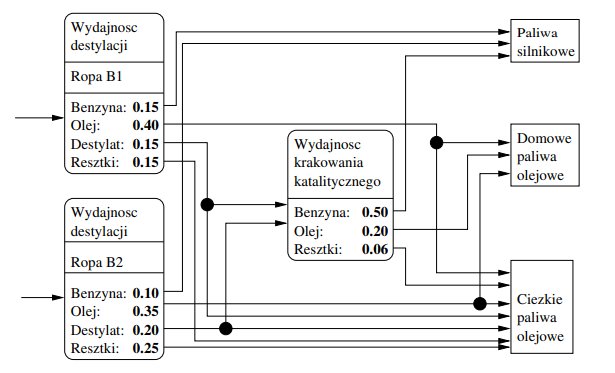
\includegraphics[width=0.65\textwidth]{rafineria.png}
    \caption{Schemat produkcji w rafinerii - z treści zadania}
    \label{fig:rafineria}
\end{figure}

\subsection{Model}
Model parametryzowany jest zbiorem rop $R$, zbiorem produktów $P$, kategorii produktów $K$ oraz zbiorem faz produkcji $F$.
Dla każdej z rop $r \in R$ zadana jest jej cena $c_r$ w dolarach, każda kategoria $k \in K$ ma przyporządkowane produkty, które ją tworzą a każda faza $f \in F$ ma określoną wydajność $w_p^f$ dla poszczególnych produktów $p \in P$ a także koszt produkcji $k_f$ w dolarach.
Produkty w ramach kategorii mogą się powtarzać ($k \subseteq P$).
Parametrem powstałych produktów jest zawartość siarki. W olejach procentowa zawartość siarki nie może przekraczać $s_{max}$. Przy produkcji oleju w danej fazie $f \in F$ z ropy $r \in R$ zawartość siarki w oleju wynosi $s_r^f$.
Dodatkowo dla każdej kategorii $k \in K$ określone jest zapotrzebowanie $z_k$ w tonach. 
Połączenia wewnątrz rafinerii zadawane są macierzami połączeń między fazami $f_1, f_2 \in F$ dla danych produktów $p \in P$ $a_{f_1,f_2,p}$, połączeń faz $f \in F$ ze zbiornikami odpowiadającymi kategoriom $k \in K$ produktów $p \in P$ $b_{f,k,p}$ oraz opisem wejść danej ropy $r \in R$ do fazy $f \in F$ $c_{r,f}$.
Zakładamy, że połączenia wewnątrz rafinerii nie tworzą cykli.

\subsubsection{Zmienne decyzyjne}
Rzeczywiste nieujemne zmienne decyzyjne opisują ilość potrzebnej ropy $r \in R$ $x_r$ w tonach oraz ilość wyprodukowanych produktów danej kategorii $k \in K$ $y_k$ w tonach.
Stan wewnątrzny rafinerii opisują także rzeczywiste nieujemne zmienne decyzyjne $z^1_{f, r, p}$ i $z^2_{f, r, p}$ opisujące ilość ropy lub produktu $p \in R \cup P$ w tonach przed i po fazie $f \in F$ dla źródła ropy $r \in R$
oraz zmienne $t^1_{f_1, k, r, p}$ i $t^2_{f_1, f_2, r, p}$ opisujące ilość produktu $p \in R \cup P$ w tonach, który powstał z ropy $r \in R$, który po fazie $f_1 \in F$ trafi do bezpośrednio do zbiornika kategorii $k \in K$ albo zostanie przetworzony w~kolejnej fazie $f_2$.

\subsubsection{Funkcja celu}
Funkcją celu jest minimalizacja kosztów produkcji: $\displaystyle \sum_{r \in R} c_r \cdot x_r + \sum_{f \in F, r \in R \atop p \in P \cup R} k_f \cdot z^1_{f, r, p}$.

\subsubsection{Ograniczenia}
\begin{itemize}
    \item wejścia ropy do rafinerii: $\displaystyle \left(\forall r \in R \right) \left(x_r = \sum_{f \in F} c_{r,f} \cdot z^1_{f, r, r} \right)$
    \item połączenia między fazami: $\displaystyle \left(\forall f_1 \in F \right)\left(\forall r \in R \right)\left(\forall p \in R \cup P \right) \sum_{f_2 \in F} a_{f_2,f_1,p} \cdot t^2_{f_2, f_1, r, p} = z^1_{f_1, r, p}$
    \item przepływ produktów przez kolejne fazy: $\displaystyle \left(\forall f \in F \right)\left(\forall r \in R \right)\left(\forall p \in P \right) \left(c_{r, f} + w_p^f \cdot \sum_{p' \in P \cup R} z^1_{f, r, p'} = z^2_{f, r, p} \right)$
    \item rozdzielanie produktów po kolejnych fazach: $\displaystyle \left(\forall f \in F \right)\left(\forall r \in R \right)\left(\forall p \in P \right) \left(z^2_{f, r, p} = \sum_{f' \in F}(t^1_{f, f', r, p} + t^2_{f, f', r, p}) \right)$
    \item zbieranie produktów w zbiornikach: $\displaystyle \left(\forall k \in K \right) \left(\sum_{f_1 \in F, r \in R \atop p \in P} t^1_{f, k, k, p} \cdot b_{f,k,p} = y_k \right)$
    \item spełnienie zapotrzebowań: $\displaystyle \left(\forall k \in K \right) \left(y_k \geq z_k \right)$
    \item limit siarki: $\displaystyle \left(\forall r \in R \right) \left((z^2_{kraking, r, olej} \cdot s_r^{kraking} + z^2_{dest1, r, olej} \cdot s_r^{dest1} + z^2_{dest2, r, olej} \cdot s_r^{dest2})  \leq s_{max} \cdot y_{p. domowe} \right)$
\end{itemize}


\subsection{Dane}
Zadane zostały zbiory:
\begin{itemize}
    \item rodzaje ropy $R = \{$ B1, B2 $\}$
    \item produkty $P = \{$ benzyna, olej, destylat, resztki $\}$
    \item kategorie produktów $K = \{$ paliwa silnikowe, paliwa domowe, paliwa ciężkie $\}$
    \item fazy produkcji $F = \{$ destylacja 1, destylacja 2, kraking $\}$
\end{itemize}
Ustalono także ceny ropy $c_{B1} = 1300$ dolarów/tonę, $c_{B2} = 1500$ dolarów/tonę, maksymalną zawartość siarki $s_{max} = 0.005$. 
Zapotrzebowanie oraz koszty i wydajność produkcji zostały przedstawione w tabelach \ref{tab:zapotrzebowanie}, \ref{tab:koszty} i \ref{tab:wydajnosc}.
Połączenie w rafinerii zadane są macierzami \ref{tab:wejscia_ropy}, \ref{tab:przeplyw_produkcji} i \ref{tab:przeplyw_do_zbiornikow}.
\begin{table}[h]
    \centering
    \begin{minipage}{0.45\textwidth}
        \centering
        \begin{tabular}{c|c}
            Produkt & Zapotrzebowanie \\
            \hline
            Paliwo silnikowe & 200000 \\
            Paliwo domowe & 400000 \\
            Paliwo ciężkie & 250000 \\
        \end{tabular}
        \caption{Zapotrzebowanie na paliwa [tony]}
        \label{tab:zapotrzebowanie}
    \end{minipage}
    \hspace{1cm}
    \begin{minipage}{0.45\textwidth}
        \centering
        \begin{tabular}{c|c}
            Proces & Koszt produkcji \\
            \hline
            Destylacja 1 & 10 \\
            Destylacja 2 & 10 \\
            Kraking & 20 \\
        \end{tabular}
        \caption{Koszty produkcji [dolary/tonę]}
        \label{tab:koszty}
    \end{minipage}
\end{table}

\begin{table}[h]
    \centering
    \begin{minipage}{0.45\textwidth}
        \centering
        \begin{tabular}{c|cccc}
            Proces & Benzyna & Olej & Destylat & Resztki \\
            \hline
            Destylacja 1 & 0.15 & 0.40 & 0.15 & 0.15 \\
            Destylacja 2 & 0.10 & 0.35 & 0.20 & 0.25 \\
            Kraking & 0.50 & 0.20 & 0.00 & 0.06 \\
        \end{tabular}
        \caption{Wydajność produkcji}
        \label{tab:wydajnosc}
    \end{minipage}
    \hfill
    \begin{minipage}{0.45\textwidth}
        \centering
        \begin{tabular}{c|cc}
            & B1 & B2 \\
            \hline
            Destylacja 1 & 1 & 0 \\
            Destylacja 2 & 0 & 1 \\
            Kraking & 0 & 0 \\
        \end{tabular}
        \caption{Wejścia ropy do procesów produkcyjnych}
        \label{tab:wejscia_ropy}
    \end{minipage}
\end{table}

\begin{table}[h!]
    \centering
    \begin{minipage}{0.45\textwidth}
        \centering
        \begin{tabular}{cccc}
            & Dest. 1 & Dest. 2 & Kraking \\
            \hline
            \hline
            \multicolumn{4}{c}{Benzyna} \\
            \hline
            Destylacja 1 & 0 & 0 & 0 \\
            Destylacja 2 & 0 & 0 & 0 \\
            Kraking & 0 & 0 & 0 \\
            \multicolumn{4}{c}{Olej} \\
            \hline
            Destylacja 1 & 0 & 0 & 0 \\
            Destylacja 2 & 0 & 0 & 0 \\
            Kraking & 0 & 0 & 0 \\
            \multicolumn{4}{c}{Destylat} \\
            \hline
            Destylacja 1 & 0 & 0 & 1 \\
            Destylacja 2 & 0 & 0 & 1 \\
            Kraking & 0 & 0 & 0 \\
            \multicolumn{4}{c}{Resztki} \\
            \hline
            Destylacja 1 & 0 & 0 & 0 \\
            Destylacja 2 & 0 & 0 & 0 \\
            Kraking & 0 & 0 & 0 \\
        \end{tabular}
        \caption{Przepływ produkcji}
        \label{tab:przeplyw_produkcji}
    \end{minipage}
    \hfill
    \begin{minipage}{0.45\textwidth}
        \centering
        \begin{tabular}{cccc}
            & P. Silnikowe & P. Domowe & P. Ciężkie \\
            \hline
            \hline
            \multicolumn{4}{c}{Benzyna} \\
            \hline
            Destylacja 1 & 1 & 0 & 0 \\
            Destylacja 2 & 1 & 0 & 0 \\
            Kraking & 1 & 0 & 0 \\
            \multicolumn{4}{c}{Olej} \\
            \hline
            Destylacja 1 & 0 & 1 & 1 \\
            Destylacja 2 & 0 & 1 & 1 \\
            Kraking & 0 & 1 & 0 \\
            \multicolumn{4}{c}{Destylat} \\
            \hline
            Destylacja 1 & 0 & 0 & 1 \\
            Destylacja 2 & 0 & 0 & 1 \\
            Kraking & 0 & 0 & 0 \\
            \multicolumn{4}{c}{Resztki} \\
            \hline
            Destylacja 1 & 0 & 0 & 1 \\
            Destylacja 2 & 0 & 0 & 1 \\
            Kraking & 0 & 0 & 1 \\
        \end{tabular}
        \caption{Przepływ do zbiorników}
        \label{tab:przeplyw_do_zbiornikow}
    \end{minipage}
\end{table}

\subsection{Wyniki}
Zapisano model programowania liniowego i wyznaczono optymalny plan produkcji. Szczegółowe wyniki przedstawiono w tabelach poniżej. Całkowity koszt produkcji wynosi 1345943600.9 dolarów.
Proste obliczenia wskazują, że otrzymane rozwiązanie jest dopuszczalne.
\begin{table}[h!]
    \centering
    \begin{tabular}{c|c} 
        \multicolumn{2}{c}{Zużycie ropy naftowej} \\ \hline
        B1 & 1026030.368764 \\ 
        B2 & 0.000000 \\ 
    \end{tabular}
    \hspace{2cm}
    \begin{tabular}{c|c} 
        \multicolumn{2}{c}{Ilość wyprodukowanych paliw} \\ \hline
        Paliwo silnikowe & 200000.000000 \\ 
        Paliwo domowe & 400000.000000 \\ 
        Paliwo ciężkie & 250000.000000 \\ 
    \end{tabular}
    \caption{Zużycie ropy naftowej oraz ilość wyprodukowanych paliw w tonach}
    \label{tab:zuzycie_i_produkcja}
\end{table}
\begin{table}[h!]
    \centering
    \begin{tabular}{c|cccc}
        Proces     & Benzyna (B1)       & Olej (B1)         & Destylat (B1)      & Resztki (B1)       \\
        \hline
        Destylacja 1& 153904.56         & 410412.15        & 153904.56         & 153904.56         \\
        Destylacja 2& 0         & 0        & 0         & 0         \\
        Kraking      & 46095.44          & 18438.18         & 0                 & 5531.45           \\
    \end{tabular}
    \caption{Szczegółowe wyniki produkcji w tonach}
    \label{tab:przeplyw_wyjscia_zbiorniki}
\end{table}

\section{Zadanie 4}
\subsection{Cel}
Celem zadania jest wybranie grup zajęciowych w taki sposób aby nie nakladały się one na siebie w czasie, uzwględniały czas na obiad, umożliwiały uczęszczanie na trening sportowy oraz nie przekraczamy określonej liczby godzin zajęć w ciągu dnia.
Dodatkowo każda grupa ma określoną wartość preferencji, których sumę chcemy zmaksymalizować. Następnie dodane zostanę ograniczenia na minimalną wartość preferencji oraz na dni w których chcemy uczęszczać na zajęcia.

\subsection{Model}
Model parametryzowany jest zbiorem dni $D$, zajęć $Z$, zbiorem grup $G$, które dotyczą każdych zajęć oraz zbiorem treningów $T$. Każda grupa $g \in G$ dotycząca danych zajęć $z \in Z$ ma przypisany początek $p^z_g$, koniec $k^z_g$ dzień $d^z_g$ oraz wartość preferencji $p^z_g$. 
Każdy trening $t \in T$ trwa od godziny $p_t$ do $k_t$ w dniu $d_t \in D$.
Przerwa obiadowa trwa od godziny $p_l$ do $k_l$ a sam obiad musi trwać co najmniej $l$ godzin.
Maksymalna liczba godzin określana jest przez $m_g$, minimalna liczba treningów w ciągu tygodnia przez $m_t$ a minimalna wartość preferencji zajęć przez $m_p$. Dni wolne od zajęć określone są przez zbiór $W \subset D$.

\subsubsection{Zmienne decyzyjne}
Binarne zmienne decyzyjne $x^z_g$, gdzie $z \in Z$, $g \in G$ określają czy grupa $g$ zostaje wybrana do zajęć $z$ a zmienne $y_t$ określają czy będzie możliwe uczęszczanie na trening $t$.

\subsubsection{Funkcja celu}
Funkcją celu jest maksymalizacja sumy wartości preferencji zajęć: $\displaystyle \sum_{z \in Z} \sum_{g \in G} p^z_g \cdot x^z_g$.

\subsubsection{Ograniczenia}
\begin{itemize}
    \item każde zajęcia muszą mieć przypisaną dokładnie jedną grupę: $\displaystyle \left(\forall z \in Z\right) \left(\sum_{g \in G} x^z_g\right) = 1$
    \item maksymalna liczba godzin w trakcie jednego dnia: $\displaystyle \left(\forall d \in D\right) \left(\sum_{z \in Z} \sum_{g \in G} \left(k^z_g - p^z_g\right) \cdot x^z_g \right)\leq m_g$
    \item odpowiednia liczba treningów: $\displaystyle \left(\sum_{t \in T} y_t\right) \geq m_t$
    \item zajęcia nie mogą na siebie nachodzić: \newline $\displaystyle \left(\forall z_1, z_2 \in Z\right) \left(\forall g_1, g_2 \in G\right) \left(z_1 \ne z_2 \land g_1 \neq g_2 \land d^{z_1}_{g_1} = d^{z_2}_{g_2} \land p^{z_1}_{g_1} \leq k^{z_2}_{g_2} \land p^{z_2}_{g_2} \leq k^{z_1}_{g_1} \right) \Rightarrow (x^{z_1}_{g_1} + x^{z_2}_{g_2}) \leq 1$
    \item trenigni nie mogą na siebie nachodzić: \newline $\displaystyle \left(\forall t_1, t_2 \in T\right) \left(t_1 \ne t_2 \land d_{t_1} = d_{t_2} \land p_{t_1} \leq k_{t_2} \land p_{t_2} \leq k_{t_1}\right) \Rightarrow (y_{t_1} + y_{t_2}) \leq 1$
    \item zajęcia i treningi nie mogą na siebie nachodzić: \newline $\displaystyle \left(\forall z \in Z\right) \left(\forall g \in G\right) \left(\forall t \in T\right) \left(d^z_g = d_t \land p^z_g \leq k_t \land p_t \leq k^z_g\right) \Rightarrow (x^z_g + y_t) \leq 1$
    % \item zapewnienie wolnego czasu na obiad: \newline $\displaystyle \left(\forall d \in D\right) \left(\sum_{z \in Z, g \in G \atop d^z_g = d} \textlbrackdbl\textlbrackdbl p^z_g < k_l \land k^z_g > p_l \textrbrackdbl\textrbrackdbl \cdot (\min(k^z_g, k_l) - \max(p^z_g, p_l)) \cdot x^z_g + \sum_{t \in T \atop d_t = d} \textlbrackdbl\textlbrackdbl p_t < k_l \land k_t > p_l \textrbrackdbl\textrbrackdbl \cdot (\min(k_t, k_l) - \max(p_t, p_l)) \cdot y_t \right)$
    \item zapewnienie wolnego czasu na obiad($\textlbrackdbl\textlbrackdbl * \textrbrackdbl\textrbrackdbl$ oznacza nawias Iversona): $\forall d \in D$:
    \begin{equation}
        \begin{split}
            \left( \sum_{z \in Z, g \in G \atop d^z_g = d} \textlbrackdbl\textlbrackdbl p^z_g < k_l \land k^z_g > p_l \textrbrackdbl\textrbrackdbl \cdot (\min(k^z_g, k_l) - \max(p^z_g, p_l)) \cdot x^z_g + \quad \quad \quad \quad \right. \\ \left.
                   \sum_{t \in T \atop d_t = d} \textlbrackdbl\textlbrackdbl p_t < k_l \land k_t > p_l \textrbrackdbl\textrbrackdbl \cdot (\min(k_t, k_l) - \max(p_t, p_l)) \cdot y_t \right) \leq k_l - p_l - l
        \end{split}
        \end{equation}
    \item zapewnienie wolnych dni: $\displaystyle (\forall z \in Z)(\forall g \in G) \left(d^z_g \in W \right) \Rightarrow x^z_g = 0$
    \item minimalna wartość preferencji: $\displaystyle \left(\forall z \in Z\right) \left(\forall g \in G\right) \left(p^z_g \geq m_p \cdot x^z_g\right)$
\end{itemize}
Najważniejszą częścią ograniczeń jest sprawdzanie nachodzenia na siebie zakresów czasowych zajęć, treningów oraz obiadu. 
Dwa przedziały $[a,b]$ oraz $[c,d]$ nachodzą na siebie wtedy i tylko wtedy gdy $a \leq d \land c \leq b$.
Dla każdych nachodzących na siebie zajęć, treningów oraz obiadu zmienne decyzyjne muszą sumować się do co najwyżej 1 co oznacze wybór jednego z nich.
Ograniczenie dotyczące czasu na obiad sprawdza czy suma czasów zajęć i treningów trwających w przerwie obiadowej jest mniejsza niż czas przerwy obiadowej pomniejszony o~czas obiadu.

\subsection{Dane}
Zadane zostały zbiory:
\begin{itemize}
    \item dni tygodnia $D = \{1,2,3,4,5\}$
    \item zajęcia $Z = \{$ Algebra, Analiza, Fizyka, Chemia Minerałów, Chemia Organiczna $\}$
    \item grupy $G = \{$ Gr1, Gr2, Gr3, Gr4 $\}$
    \item treningi $T = \{$ Tr1, Tr2, Tr3 $\}$
    \item dni wolne $W = \{3,5\}$
\end{itemize}
oraz parametry opisujące wartości preferencji zajęc oraz czasy odbywania się zajęć i treningów - opisują to tabele \ref{tab:preferencje}, \ref{tab:zajecia} i \ref{tab:treningi}.
Obiad mógł odbywać się między $p_l = \textit{12:00}$ a $k_l = \textit{14:00}$ a minimalny czas obiadu wynosi $l = \textit{1}$ godziny. Zapewniony powinien być conajmniej jeden trening w tygodniu $m_t = \textit{1}$ oraz nie więcej niż $m_g = \textit{4}$ godzin zajęć dziennie. Minimalna wartość preferencji zajęć wynosi $m_p = \textit{5}$.
\begin{table}[h]
    \centering
    \begin{tabular}{l|cccc|cccc|cccc}
        & \multicolumn{4}{c}{Dni zajęć} & \multicolumn{4}{c}{Początki zajęć} & \multicolumn{4}{c}{Końce zajęć} \\
        & Gr1 & Gr2 & Gr3 & Gr4 & Gr1 & Gr2 & Gr3 & Gr4 & Gr1 & Gr2 & Gr3 & Gr4 \\
        \hline
        Algebra & 1 & 2 & 3 & 3 & 13 & 10 & 10 & 11 & 15 & 12 & 12 & 13 \\
        Analiza & 1 & 2 & 3 & 4 & 13 & 10 & 11 & 8 & 15 & 12 & 13 & 10 \\
        Fizyka & 2 & 2 & 4 & 4 & 8 & 10 & 15 & 17 & 11 & 13 & 18 & 20 \\
        Chemia Mineralow & 1 & 1 & 4 & 5 & 8 & 8 & 13 & 13 & 10 & 10 & 15 & 15 \\
        Chemia Organiczna & 1 & 1 & 5 & 5 & 9 & 10.5 & 11 & 13 & 10.5 & 12 & 12.5 & 14.5 \\
    \end{tabular}
    \caption{Tabela przedstawiająca dni zajęć, początki i końce zajęć dla różnych grup}
    \label{tab:zajecia}
\end{table}

\begin{table}[h]
    \centering
    \begin{minipage}{0.45\textwidth}
        \centering
        \begin{tabular}{l|cccc}
            & \multicolumn{4}{c}{Preferencje} \\
            & Gr1 & Gr2 & Gr3 & Gr4 \\
            \hline
            Algebra & 5 & 4 & 10 & 5 \\
            Analiza & 4 & 4 & 5 & 6 \\
            Fizyka & 3 & 5 & 7 & 8 \\
            Chemia Mineralow & 10 & 10 & 7 & 5 \\
            Chemia Organiczna & 0 & 5 & 3 & 4 \\
        \end{tabular}
        \caption{Tabela przedstawiająca preferencje dla różnych grup}
        \label{tab:preferencje}
    \end{minipage}
    \hspace{0.5cm}
    \begin{minipage}{0.45\textwidth}
        \centering
        \begin{tabular}{l|ccc}
            & \multicolumn{3}{c}{Treningi} \\
            & Dni & Początki & Końce \\
            \hline
            Tr1 & 1 & 13 & 15 \\
            Tr2 & 3 & 11 & 13 \\
            Tr3 & 3 & 13 & 15 \\
        \end{tabular}
        \caption{Tabela przedstawiająca dni treningów, ich początki i końce}
        \label{tab:treningi}
    \end{minipage}
\end{table}

\newpage

\subsection{Wyniki}
Zapisano model programowania liniowego i wygenerowano grupy zajęciowe i treningi. 
Rozpatrzono dane bez zadanych dni wolnych i minimalnej wartości preferencji. Suma preferencji wyniosła odpowiednio $37$ i $28$. Wybrane zajęcia przedstawiono w tabeli \ref{tab:zajecia_trening}.
\begin{table}[h]
    \centering
    \begin{tabular}{lcc}
        & \multicolumn{2}{c}{Grupa} \\
        & Wersja 1 & Wersja 2 \\
        \hline
        Zajęcia Algebra & Gr3 & Gr1 \\
        Zajęcia Analiza & Gr2 & Gr4 \\
        Zajęcia Fizyka & Gr4 & Gr2 \\
        Zajęcia Chemia Mineralow & Gr1 & Gr3 \\
        Zajęcia Chemia Organiczna & Gr2 & Gr2 \\
        Trening & Tr1 & Tr2 \\
    \end{tabular}
    \caption{Tabela przedstawiająca przypisane grupy do zajęć i wybrany trening w obu wersjach danych}
    \label{tab:zajecia_trening}
\end{table}

Łatwo sprawdzić, że wygenerowane rozwiązania są dopuszczalne.

\end{document}